%This Source Code Form is subject to the terms of the Mozilla Public License, v. 2.0. If a copy of the MPL was not distributed with this file, You can obtain one at http://mozilla.org/MPL/2.0/.
%%%
% Minimal working example for the beamer theme "minimal"
% Last Update: 15-02-2017
% In case of questions/problems/proposals you can write, call or visit me
% http://cs.uni-paderborn.de/cuk/personal/sascha-brauer/
%%%
\documentclass{beamer}

%% Use the handout option to color-invert decorations
\usetheme{minimal}

\usepackage{color}
\usepackage{lmodern}
\usepackage{outlines}

\usepackage{graphicx}
\usepackage{media9}

\title{Thema 7\\Hypertext-Systeme 1}

\author{Kevin Haack}
\institute{Universität Paderborn}

\date{\today}

\setbeamertemplate{section in toc}[ball unnumbered]


\begin{document}

\begin{frame}
  \titlepage
\end{frame}

\begin{frame}{Übersicht}
\tableofcontents
\end{frame}

\begin{frame}{Übersicht}
	\begin{figure}[htbp]
		\centering
		
\includegraphics[width=0.65\textwidth]{images/philosoraptor}
	\end{figure}
\end{frame}

\section{Abgrenzung}
\begin{frame}{Abgrenzung}
	\begin{itemize}
		\item Memex (1945)
		\item Hypertext-Systeme 2
		\item closed hypertext systems
		\item Beschränkung auf Hypertextfunktionen und Benutzung
		\item Keine Kategorisierung
	\end{itemize}
\end{frame}

\section{Geschichte}
\begin{frame}{Geschichte}
\begin{itemize}
	\item 1945: \textbf{MEMEX / As we may think}
	\item 1960: \textbf{Xanadu}
	\item 1967: \textbf{HES}
	\item 1968: The mother of all demos, \textbf{FRESS}, \textbf{NLS}
	\item 1980: ENQUIRE am CERN
	\item 1982: Guide
	\item 1983: \textbf{HyperTIES}
	\item 1985: \textbf{Document Examiner}
	\item 1987: HyperCard für MAC
	\item 1988: Hypertext on Hypertext
	\item 1989: Information Management: a Proposal
	\item 1990: WinHelp, Storyspace, Hypertext hands-on!
\end{itemize}
\end{frame}

\section{Struktur}

\begin{frame}{Struktur}
\begin{itemize}
	\item Projekt / Anwendung
	\item Autor
	\item Zeitliche Einordnung
	\item Zielgruppe
	\item Userinterface / Bedienmöglichkeiten
	\item Links / Strukturen
\end{itemize}
\end{frame}

\section{Systeme}

\begin{frame}
\frametitle{Memex}
\begin{itemize}
	\item maschinellen Unterstützung des menschlichen Gedächtnisses und des assoziativen Denkens
	\item Schreibtisch
	\item Kombination von elektromechanischen Kontrollen und Mikrofilmgeräten
	\item Illustrationen im Life Magazine 19. November 1945
	\item kopfmontierte Kamera sowie eine Schreibmaschine, die über Spracherkennung verfügen und die Texte mittels Sprachsynthese vorlesen soll. 
\end{itemize}
\end{frame}

\begin{frame}
	\frametitle{Memex}
	\framesubtitle{Funktionen}
	\begin{itemize}

		\item Seiten durch Verknüpfungen (associations) aufeinander verweisen zu lassen.
		\item mit Hebeln vor- und zurückblättern sowie Dokumente speichern und wieder aufrufen
		\item berührungssensitiven Bildschirmen 

	\end{itemize}

	\begin{figure}[htbp]
		\centering
		\includegraphics[width=0.4\textwidth]{images/memex}
	\end{figure}

\end{frame}

\begin{frame}
\frametitle{NLS: oN-Line System}
\begin{itemize}
	\item 1960er (1968 "the mother of all demos")
	\item Online nicht im WWW, sondern interaktiv
	\item Doug Engelbart, Stanford Research Institute
	\item Ziel war es "den menschlichen Intellekt zu erweitern"
	\begin{itemize}
		\item Computer zur direkten Interaktion
		\item Computer Bildschirme zur Darstellung von Text
	\end{itemize}
	\item Terminal
\end{itemize}

\begin{figure}[htbp]
	\centering
	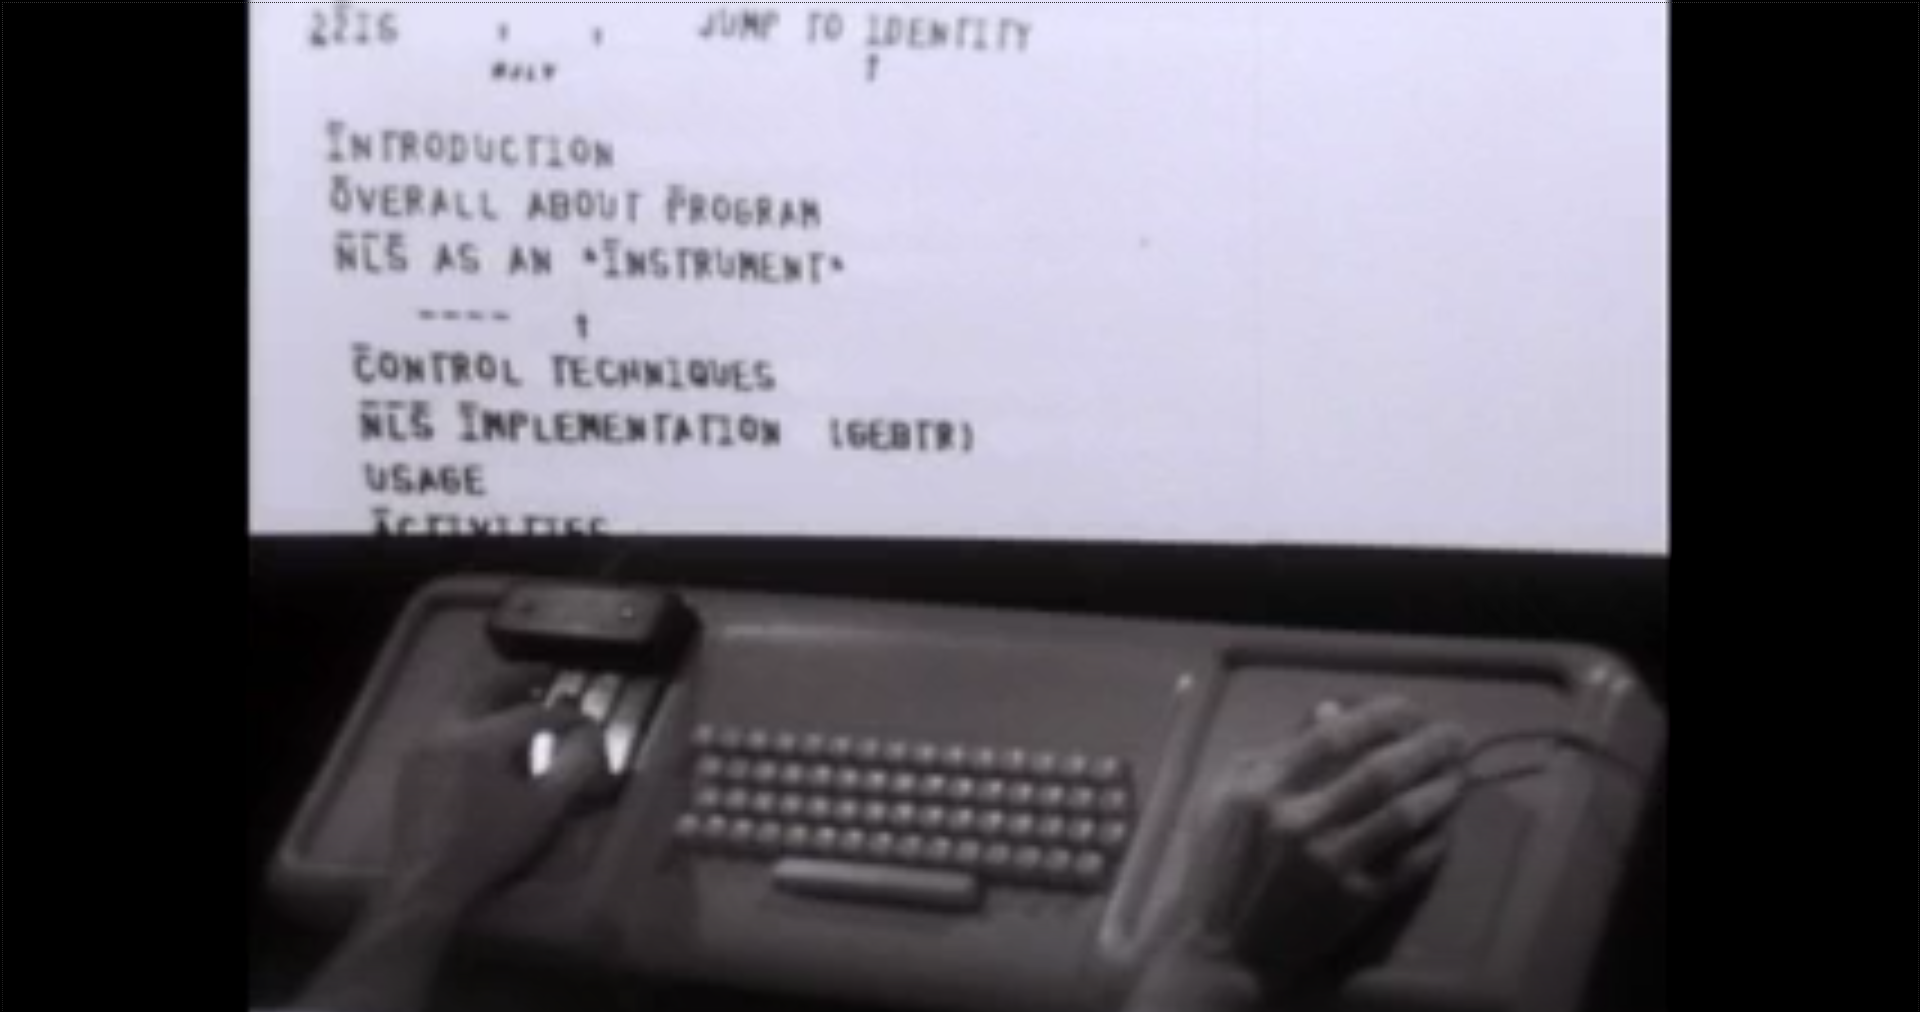
\includegraphics[width=0.7\textwidth]{images/nls}
\end{figure}

\end{frame}

\begin{frame}
\frametitle{NLS: oN-Line System}
\framesubtitle{Funktionen}
	\begin{itemize}
		\item Userinterface / Bedienmöglichkeiten
		\begin{itemize}
			\item Maus
			\item 5-Finger Tastatur
			\item Interaktives Textbearbeiten
		\end{itemize}
		\item Links / Strukturen
		\begin{itemize}
			\item Dokumente sind hierarchische strukturiert
			\item Jedes Segment hat eine ID
			\item Jede ID kann verlinkt werden
			\item Labels können verlinkt werden
		\end{itemize}
	\end{itemize}
\end{frame}

\begin{frame}
\frametitle{HES: Hypertext Editing System}
\begin{itemize}
	\item 1967
	\item Andries van Dam und Ted Nelson, Brown University
	\item IBM/360 Model 50 Mainframe
	\item Dokumentation der Apollo Missionen, NASA
\end{itemize}

\begin{figure}[htbp]
	\centering
	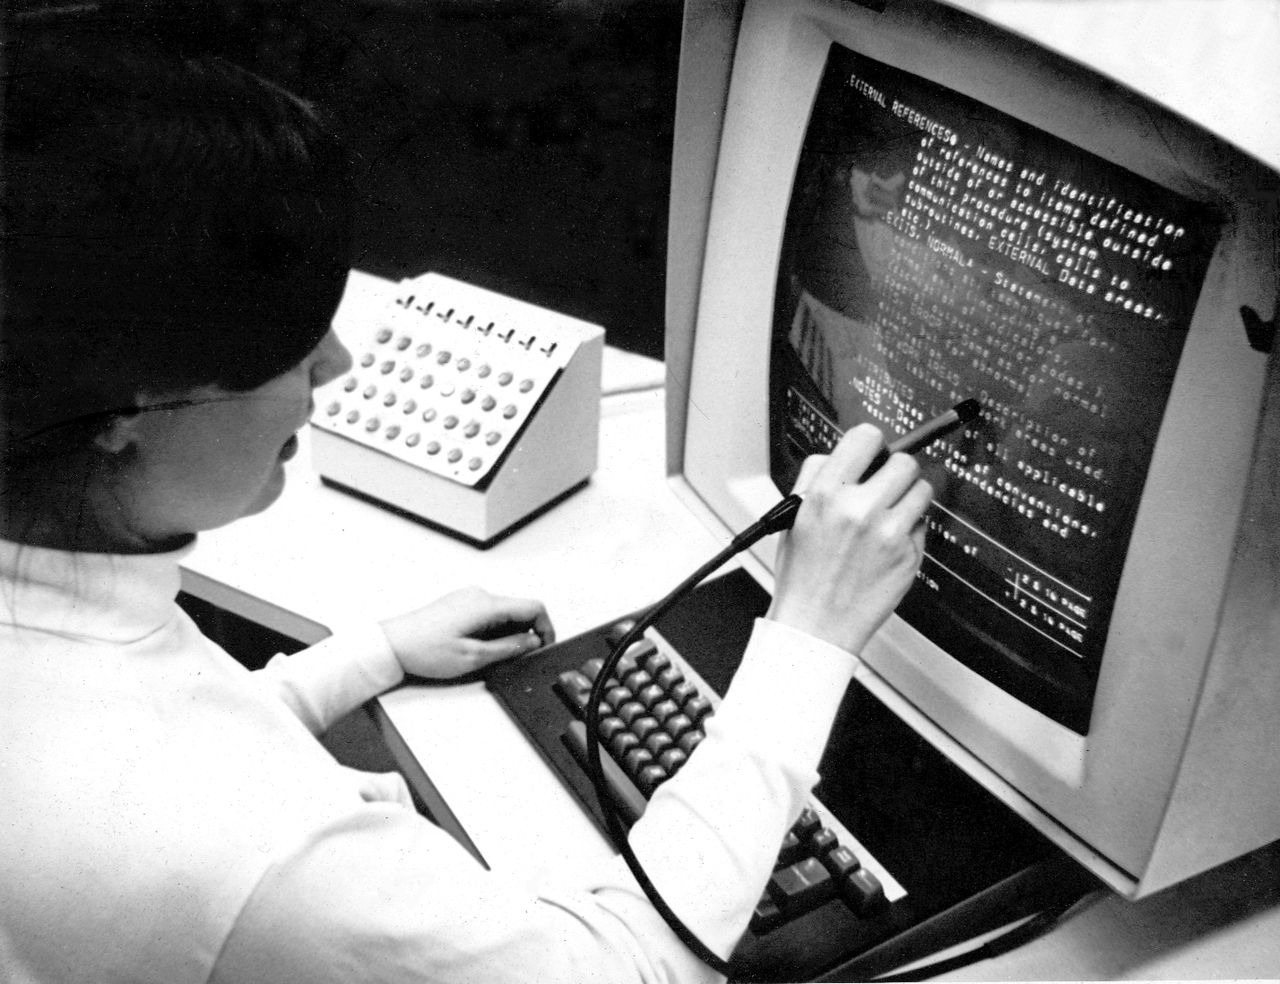
\includegraphics[width=0.40\textwidth]{images/hes}
\end{figure}

\end{frame}

\begin{frame}
\frametitle{HES: Hypertext Editing System}
\framesubtitle{Funktionen}
	\begin{itemize}
		\item Userinterface / Bedienmöglichkeiten
		\begin{itemize}
			\item Lightpenning und Tastatur
			\item Graph Darstellung
		\end{itemize}
		\item Links / Strukturen
		\begin{itemize}
			\item Kontrollinformationen für eine lineare Darstellung
			\item Pointer zu Text Fragmenten
			\item Textpassagen mit Labels referenzierbar
		\end{itemize}
	\end{itemize}
\end{frame}

\begin{frame}
\frametitle{FRESS: File Retrieval and Editing System}
\framesubtitle{Funktionen}
\begin{itemize}
	\item 1968
	\item Andries van Dam, Bob Wallace und Studenten
	\item Kommerzielle Betriebssysteme
	\item Weiterentwicklung von HES
	\item Userinterface / Bedienmöglichkeiten
	\begin{itemize}
		\item Backtrack durch die Links
		\item Windows
		\item UNDO Feature
		\item Auf PDS-1 (Minicomputer): Light Pen und Fußpedal
	\end{itemize}
	\item Links / Strukturen
	\begin{itemize}
		\item One-way Links (tag)
		\item Bi-direktionale Links (jumps)
		\item Unbegrenzte Dokumentgrößen
	\end{itemize}
\end{itemize}
\end{frame}

\begin{frame}
\frametitle{Xanadu}
\begin{itemize}
	\item 1960
	\item Langzeitprojekt (Open source in 1999)
	\item Ted Nelson
	\item mehr Framework als Programm
	\item bestehend aus Prototypen und Modelle
	\item "docuverse" - ein elektronische universale Bibliothek
\end{itemize}

\begin{figure}[htbp]
	\centering
	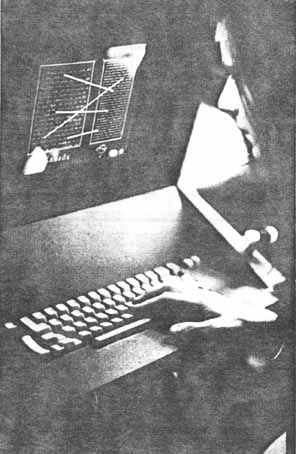
\includegraphics[width=0.22\textwidth]{images/xanadu}
\end{figure}

\end{frame}

\begin{frame}
\frametitle{Xanadu}
\framesubtitle{Funktionen}
\begin{itemize}
	\item Userinterface / Bedienmöglichkeiten
	\begin{itemize}
		\item xxxxx
	\end{itemize}
	\item Links / Strukturen
	\begin{itemize}
		\item Kommentare, Notizen und Verknüpfungen innerhalb der Dokumente zu anderen Dokumenten
	\end{itemize}
\end{itemize}
\end{frame}

\begin{frame}
\frametitle{Document Examiner}
\begin{itemize}
	\item Document Examiner: Delivery Interface for Hypertext Documents [Walker 87, p. 307]
	\item inspired by Doug Engelbart NLS
	\item record. It has a title and contains the description
	\item unique identifier
	\item book metaphor. A document-like flow of text, assembling a sequence of records into a single window
	\item Inclusion, Precis, Crossref, Implicit[Walker 87, p. 310]
	\item four panes. The content area, the Candidates and Bookmarks pane and the command region below.
	\item A click on any link does not immediately jump to the destination; instead the link is added to a list of candidates
	\item bookmarks 
	\item necessity to integrate annotations with versioning
\end{itemize}

\end{frame}
\begin{frame}
\frametitle{HyperTIES}
\begin{itemize}
	\item 1983
	\item Ben Shneiderman, University of Maryland, College Park
	\item "Simplified approach in browsing the hypertext"
	\item MS-DOS
\end{itemize}

\begin{figure}[htbp]
	\centering
	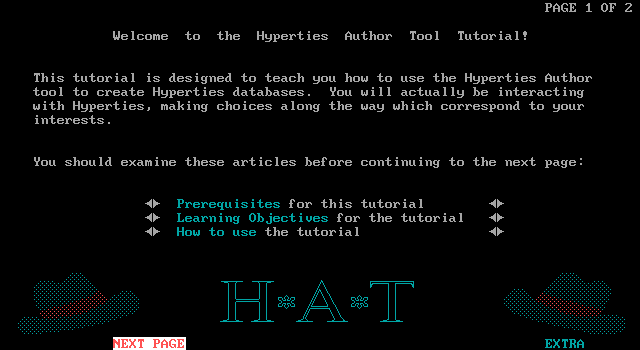
\includegraphics[width=0.7\textwidth]{images/hyperties}
\end{figure}

\end{frame}

\begin{frame}
\frametitle{HyperTIES}
\framesubtitle{Funktionen}
	\begin{itemize}
		\item Userinterface / Bedienmöglichkeiten
		\begin{itemize}
			\item Mausklick
			\item Touch Support 
			\item Pfeiltasten
		\end{itemize}
		\item Links / Strukturen
		\begin{itemize}
			\item In Artikel mit Titel und Kurzbeschreibung gegliedert
			\item Titel dient als Linktext
			\item Kurzbeschreibung dient als Preview
		\end{itemize}
	\end{itemize}
\end{frame}
%\begin{frame}
\frametitle{HyperCard}
\begin{itemize}
	\item rectangular areas on top of the text layer
\end{itemize}

\end{frame}



%\begin{frame}
\frametitle{Storyspace}
\begin{itemize}
	\item 1990 by Mark Bernstein
	\item Macintosh (Portierung für Windows)
	\item Hyperlinks do not have to be coded, they are created and directly manipulated with the mouse
	\item diagram mode visually reveals the logical structure of arguments
	\item network of writing spaces
	\item nodes inside a writing space can link to any other writing space
	\item Images can be placed into the flow of text
	\item Links are not highlighted
	\item links can point to several targets at the same time
	\item conditions to links
\end{itemize}

\end{frame}
%\begin{frame}
\frametitle{WinHelp}
\begin{itemize}
	\item 1990
	\item Microsoft Windows 3.0, entfernt in Windows Vista
	\item basierend auf RTF
\end{itemize}

\end{frame}

\begin{frame}
\frametitle{WinHelp}
\framesubtitle{Funktionen}
	\begin{itemize}
		\item Userinterface / Bedienmöglichkeiten
		\begin{itemize}
			\item xxx
		\end{itemize}
		\item Links / Strukturen
		\begin{itemize}
			\item Themen sind getrennt durch Seitenumbrüche
			\item Themen enthalten Fußnoten für den Compiler 
		\end{itemize}
	\end{itemize}
\end{frame}



\section{Zusammenfassung}
\begin{frame}{Zusammenfassung}
	\begin{itemize}
		\item 
	\end{itemize}
\end{frame}

\begin{frame}{}
	\begin{figure}[htbp]
		\centering
		
\includegraphics[width=1.0\textwidth]{images/success}
	\end{figure}
\end{frame}

\end{document}